\documentclass{article}

% if you need to pass options to natbib, use, e.g.:
%     \PassOptionsToPackage{numbers, compress}{natbib}
% before loading neurips_2019

% ready for submission
% \usepackage{neurips_2019}

% to compile a preprint version, e.g., for submission to arXiv, add add the
% [preprint] option:
%     \usepackage[preprint]{neurips_2019}

\usepackage[final]{neurips_2019}
% to compile a camera-ready version, add the [final] option, e.g.:
% to avoid loading the natbib package, add option nonatbib:
%     \usepackage[nonatbib]{neurips_2019}
\usepackage{multirow}
\usepackage[utf8]{inputenc} % allow utf-8 input
\usepackage[T1]{fontenc}    % use 8-bit T1 fonts
\usepackage{hyperref}       % hyperlinks
\usepackage{url}            % simple URL typesetting
\usepackage{booktabs}       % professional-quality tables
\usepackage{amsfonts}       % blackboard math symbols
\usepackage{nicefrac}       % compact symbols for 1/2, etc.
\usepackage{microtype}      % microtypography
\usepackage{graphicx}
\usepackage{float}

\title{

G-Research Crypto Forecasting}

% The \author macro works with any number of authors. There are two commands
% used to separate the names and addresses of multiple authors: \And and \AND.
%
% Using \And between authors leaves it to LaTeX to determine where to break the
% lines. Using \AND forces a line break at that point. So, if LaTeX puts 3 of 4
% authors names on the first line, and the last on the second line, try using
% \AND instead of \And before the third author name.

\author{%
  Fu Yang \\
  21029346\\
  \texttt{yfubo@connect.ust.hk} \\
  \And
  Luo Yuqing \\
  20582315\\
  \texttt{yluobb@connect.ust.hk} \\
  \AND
  Wang Jinyuan \\
  21028990\\
  \texttt{jwangiy@connect.ust.hk} \\
  \And
  Wang Tong \\
  20905737\\
  \texttt{twangce@connect.hk} \\
}

\begin{document}

\maketitle

\begin{abstract}
This report discusses the application of the machine learning techniques in the G-Research Crypto Forecasting competition on Kaggle, which aims to predict the future returns for 14 commonly traded cryptocurrencies. We analyze the basic features of the dataset and the conduct analysis on the statistical characteristics of the time series data, including stationarity, autoregression and decomposition. To fully utilize the data, we use the pre-implemented functions provided by TALib for feature engineering. Due to the highly volatile and non-stationary nature of the data, we choose LightGBM for this project and perform various train-test-validation splits to avoid overfitting and the model is evaluated on a weighted version of the Pearson correlation coefficient. This report is divided into five parts, including Introduction, Data, Statistical analysis, LightGBM modeling, and Performance evaluation. 


\end{abstract}

\section{Introduction}

Cryptocurrency markets have experienced a surge in popularity and trading volume in recent years. Considering their highly volatile nature, they present both lucrative opportunities and considerable risks for investors. In light of this, G-Research, Europe's leading quantitative finance research firm, has organized a Kaggle challenge to forecast the short term returns of 14 commonly traded cryptocurrencies. In the context of this competition, we employ various machine learning frameworks and models to enhance the accuracy of our prediction models. [1]


\section{Data}
\subsection{Data description}

The training dataset contains historical minute-by-minute trading data for 14 frequently traded crypto assets. The data covers the time period from January 2018 to September 2021 and description of features provided are shown in the table below. 


\begin{figure}[H]
	\centering
	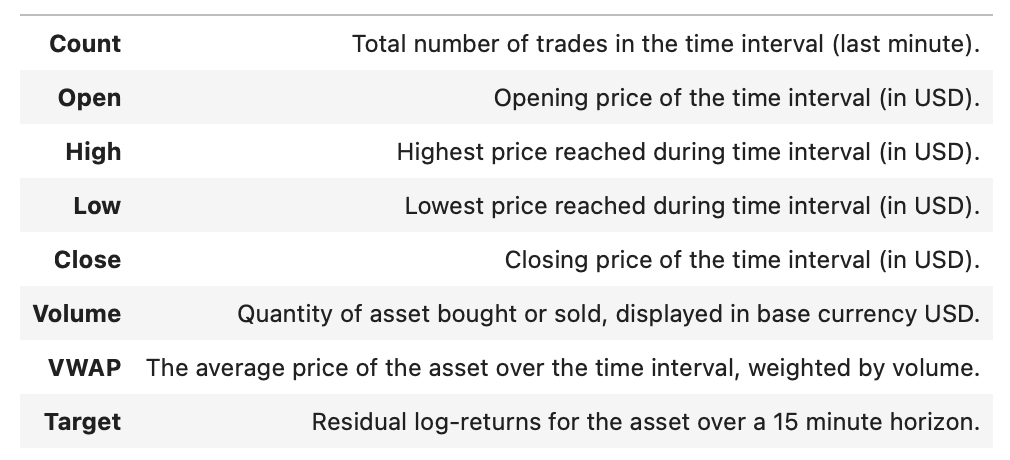
\includegraphics[width=0.8\textwidth]{Data/Feature Description.png}
	\caption{Description of features}
\end{figure}

\subsection{Data exploration}

\subsubsection{Data visualizaiton}
To gain a better understanding of the data, we follow the tutorial and visualize the trading data for the last day of Bitcoin using a candlestick bar chart. The figure depicting this visualization is shown below.

\begin{figure}[H]
	\centering
	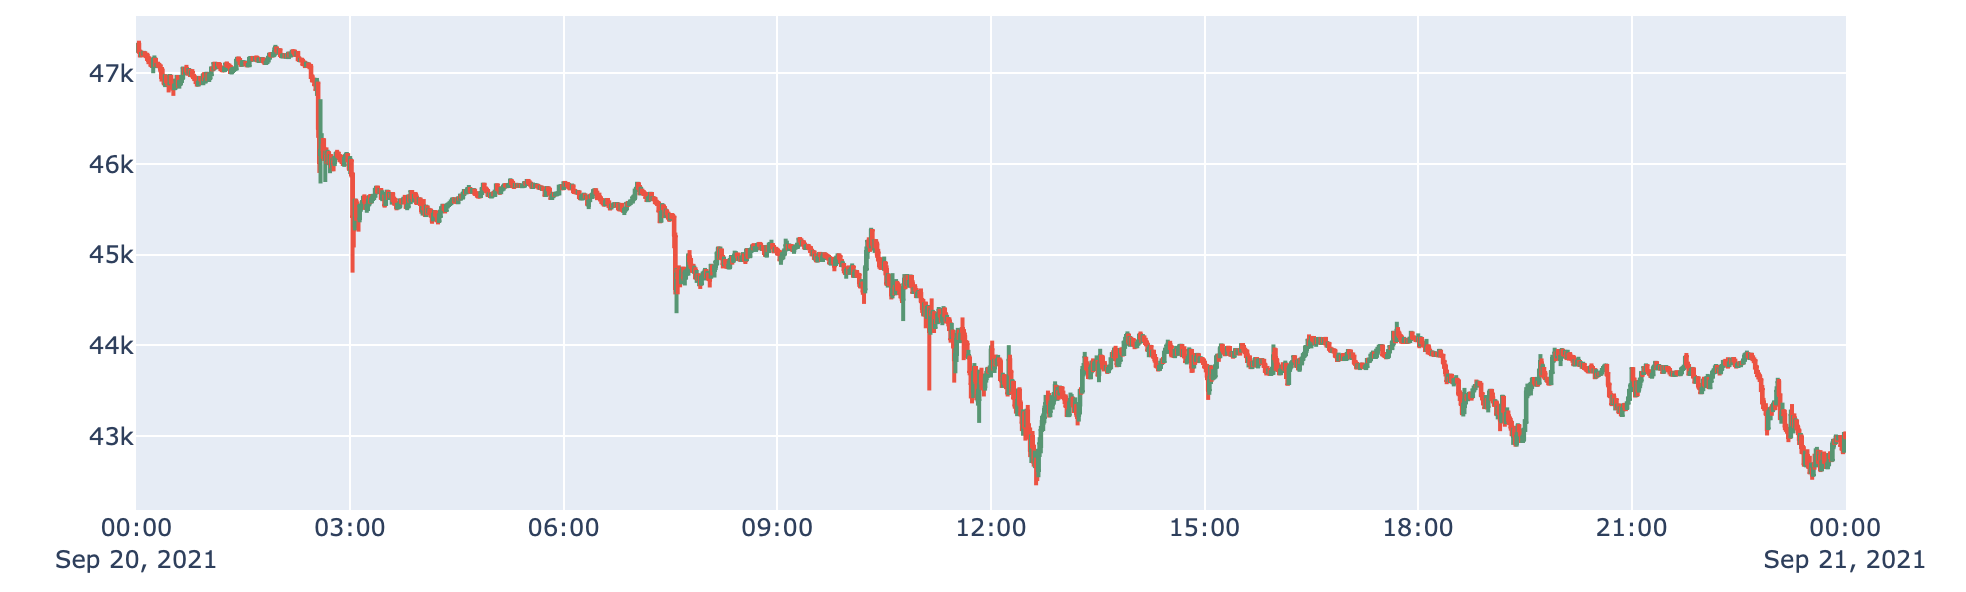
\includegraphics[width=0.8\textwidth]{Data/Visualization of Bitcoin price.png}
	\caption{Visualization of Bitcoin price}
\end{figure}

\subsubsection{Missing value}
We check for missing values in the data and find that, apart from the target variable, there are missing values in the other columns. Specifically, if there is no transaction in a particular minute, no timestamp would be recorded, resulting in gaps in the data. The number of rows for each of the 14 cryptocurrencies is shown in the figure below. We apply different approaches to handle missing values in the following sections.

\begin{figure}[H]
	\centering
	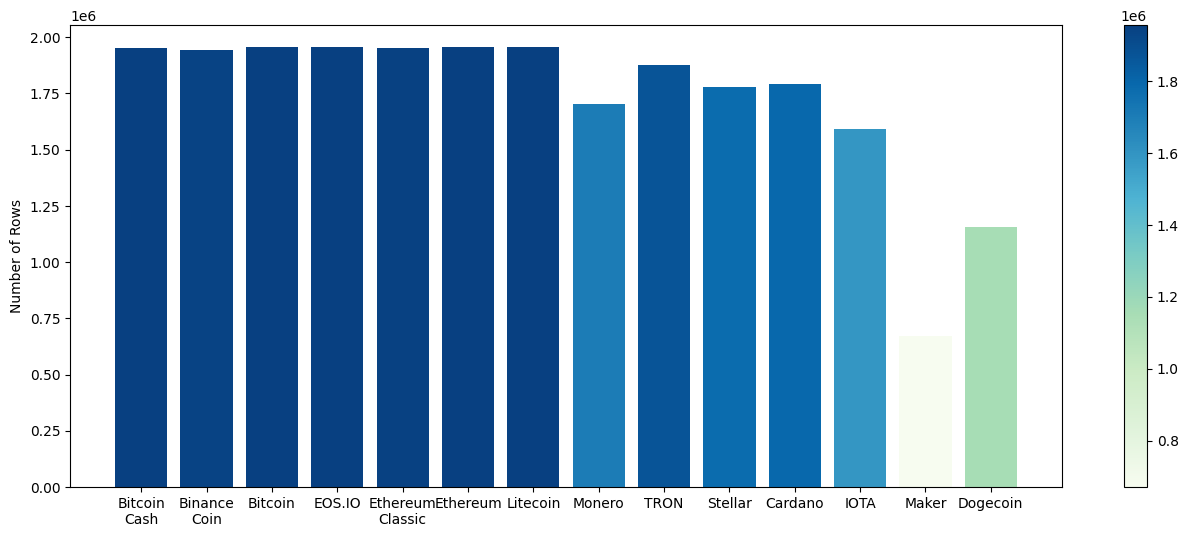
\includegraphics[width=0.8\textwidth]{Data/Number.png}
	\caption{Number of entries for each crypto currency}
\end{figure}

\subsection{Feature engineering}
To fully leverage the trading data and extract valuable insights, we utilize the pre-implemented functions provided by the Technical Analysis Library (TALib) to generate a diverse set of technical indicators. We select 45 indicators across different categories, including trend, momentum, volatility, volume, and price. 

The process of generating these features is performed dynamically, allowing for flexibility and adaptability. The method for handling missing values is set as a hyperparameter and this enables us to explore and evaluate various approaches. 

\section{Statistical analysis}
Cryptocurrency price movements are represented as time series data and it is crucial to comprehend its statistical features to select an appropriate machine learning model. We perform statistical analysis on stationarity, autocorrelation, and decomposition for further analysis.

In our analysis, we specifically focus on the closing prices from the provided trading data. For missing values, we employ a forward filling approach, which fills the gaps with the previous valid value, ensuring data completeness.

\subsection{Stationarity}
Stationarity refers to a statistical property of a time series where the statistical properties of the data do not change over time and it is a prerequisite condition for various analytical tools and models.

We apply the Augmented Dickey-Fuller (ADF) test for unit roots to assess the stationarity of the trading data. The null hypothesis of nonstationarity is tested at a significance level of 5\%. Due to the limited computational power on Kaggle and potential noise in minute frequency data, we use the average close price for each hour to conduct this test. The results for all 14 cryptocurrencies are shown in the table below.

\begin{figure}[H]
	\centering
	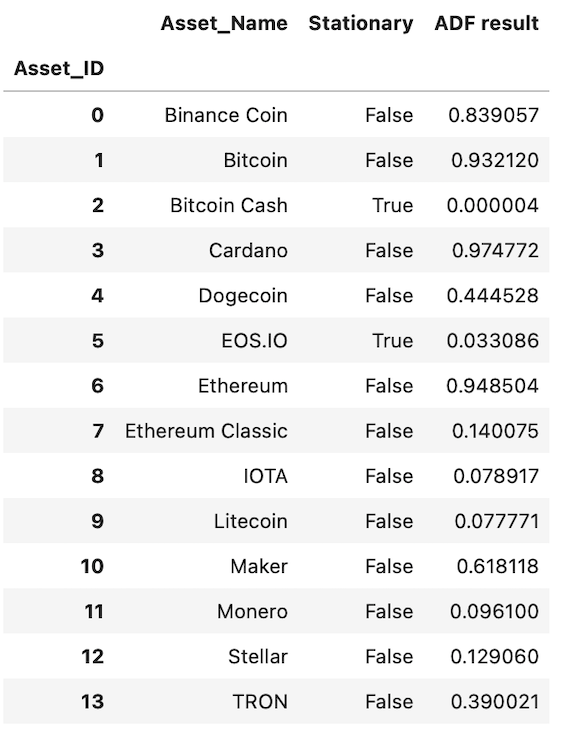
\includegraphics[width=0.5\textwidth, height=8cm]{Data/ADF test result.png}
	\caption{Number of entries for each crypto currency}
\end{figure}

The result indicates that only Bitcoin Cash and EOS.IO exhibit stationary behavior, while several other currencies show remarkably high p-values, exceeding 0.9. We should maintain consistency in the model applied to all assets, and based on these results, the overall environment is highly non-stationary.

\subsection{Autocorrelation}

Autocorrelation refers to the correlation between a variable and its lagged values and here we utilize it to analyze the pattern and trend between historical trading data and future return. We employ the partial autocorrelation function (PACF) on the trading data to control the effects of intermediate legs and calculate direct correlation between the variable and each specific lag. The result obtained for Bitcoin is presented below, and similar patterns are observed for other cryptocurrencies as well.

\begin{figure}[H]
	\centering
	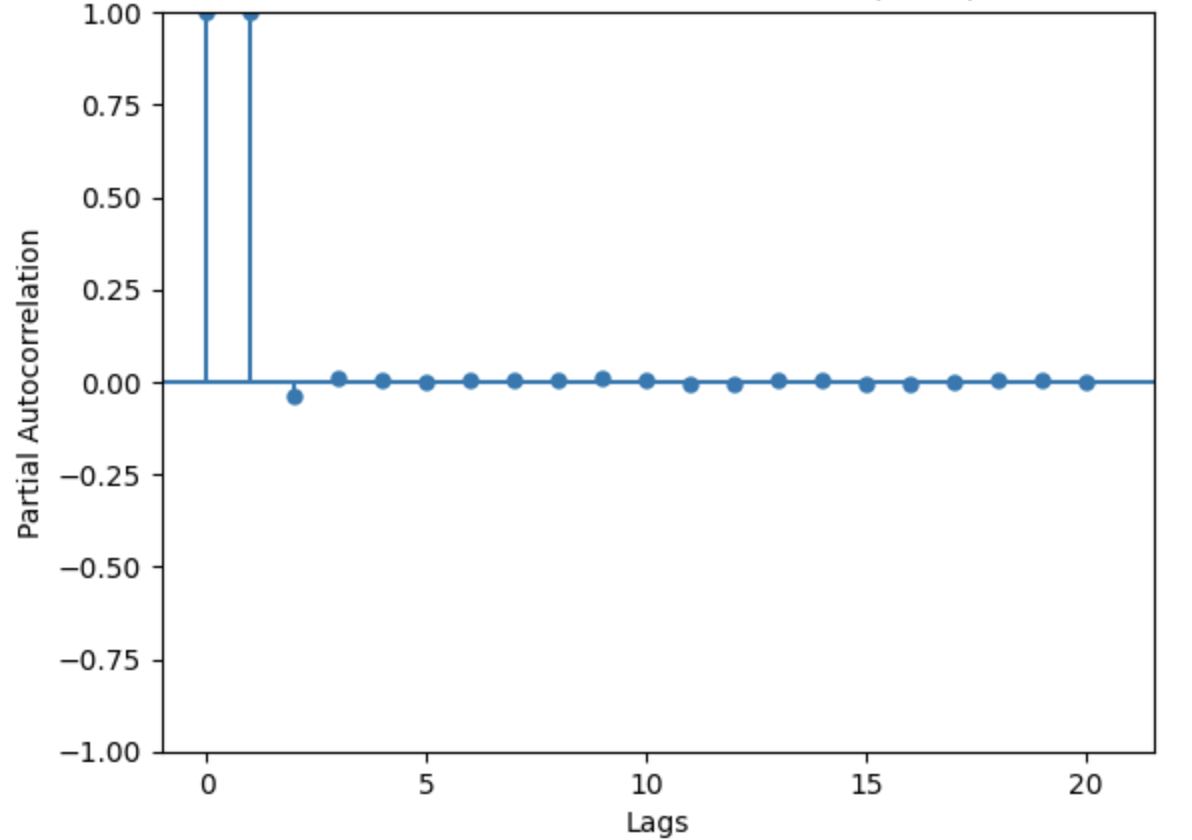
\includegraphics[width=0.7\textwidth, height=6cm]{Data/PACF plot.png}
	\caption{PACF for Bitcoin}
\end{figure}

The PACF plot shows a strong correlation between the value and its first lag, indicating the possibility of an AR(1) process. However, since the stationarity test fails for most crypto assets, AR models are not suitable for fitting the data.

\subsection{Decomposition}

We apply seasonal and trend decomposition using loess (STL) on the trading data and separate it into trend, seasonality, and residual. Trend represents the long term pattern of the time series and seasonality captures predictable variations that occur periodically. Residual is the random and irregular fluctuations  that exhibit no discernible patterns. The result obtained for Bitcoin is presented below and other cryptocurrencies have similar patterns.

\begin{figure}[H]
	\centering
	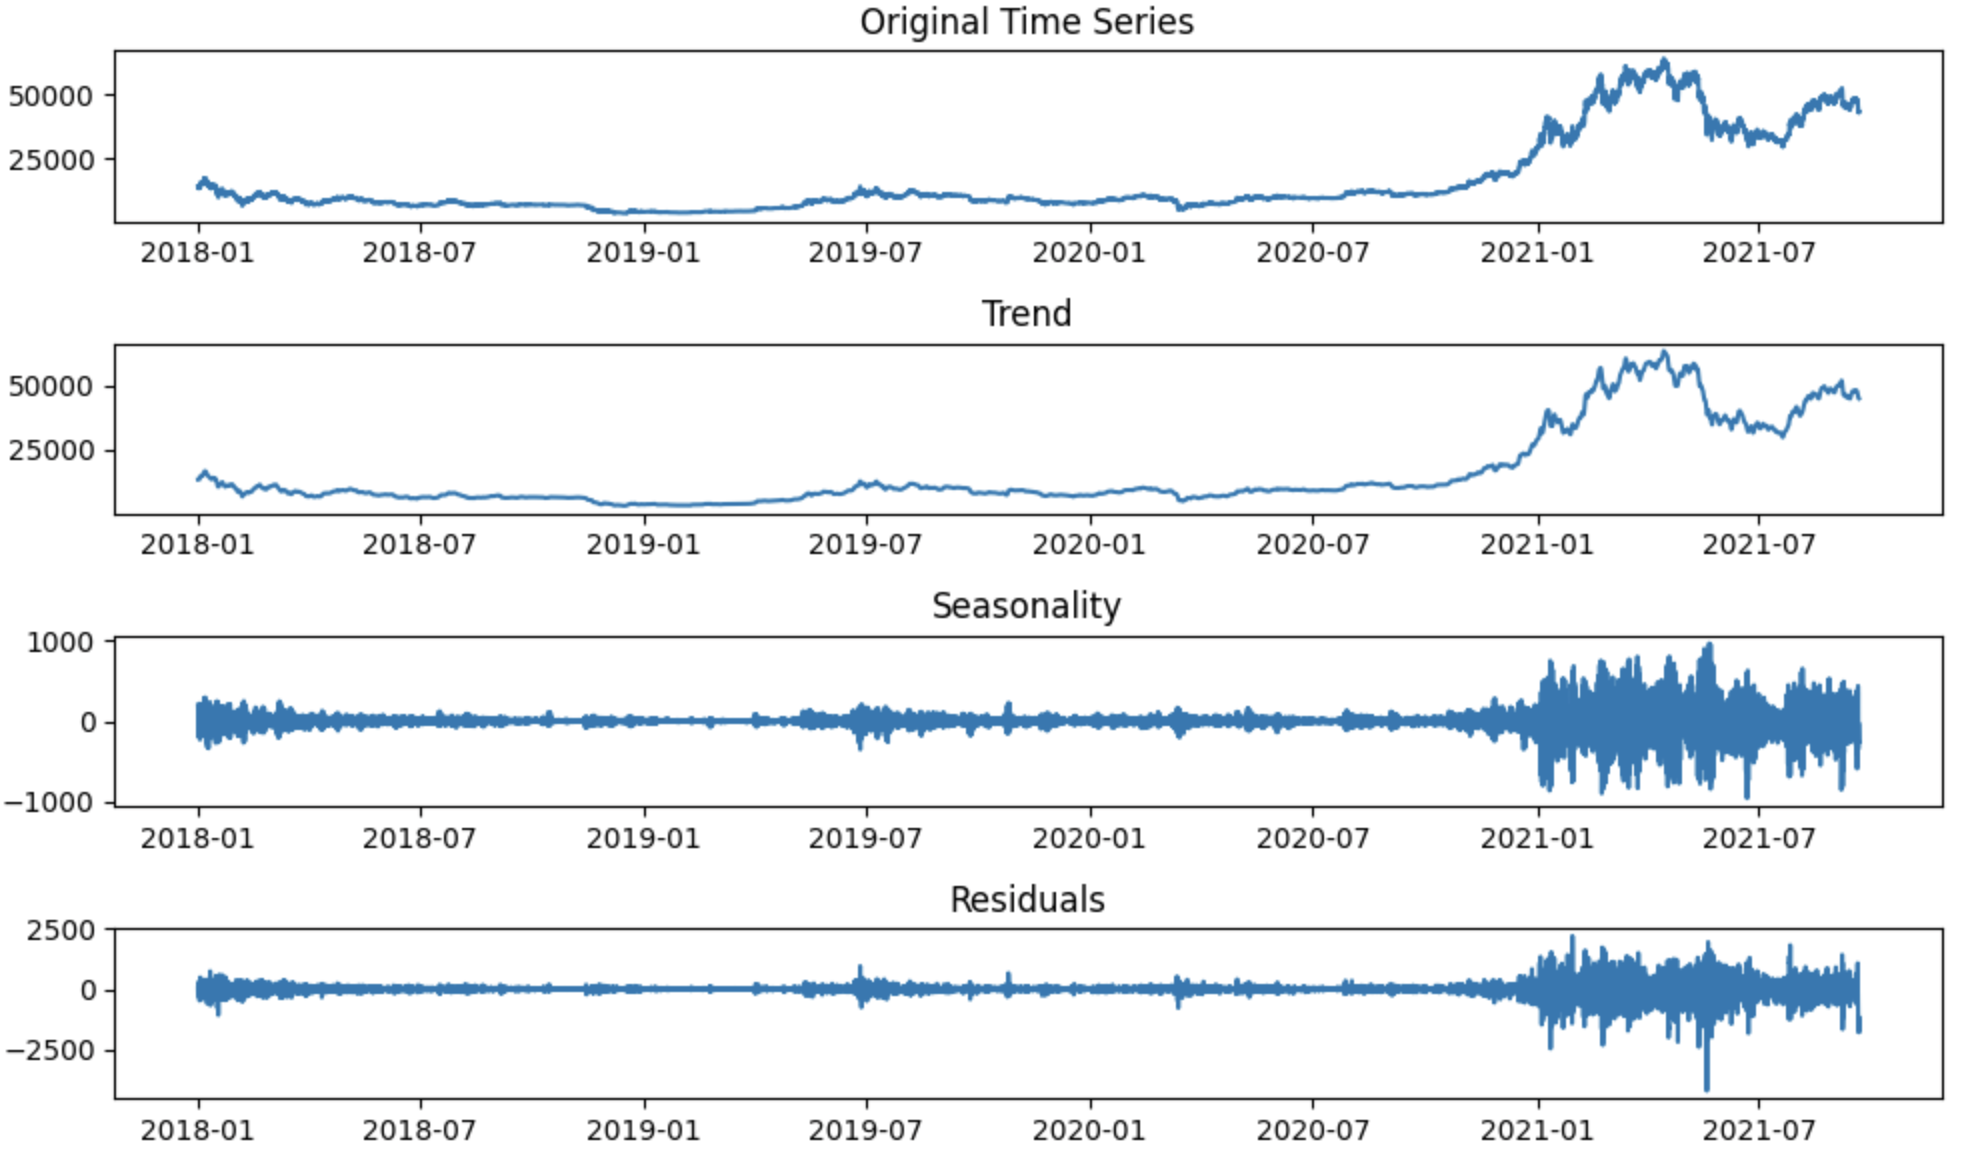
\includegraphics[width=0.8\textwidth]{Data/STL.png}
	\caption{STL for Bitcoin}
\end{figure}

Prior to 2021, the trend component exhibited a relatively stable pattern, with minimal fluctuations. The seasonality component displayed small variations, and the residual component had relatively low values, suggesting limited unexplained variation. However, a significant shift occurred after 2021. The trend component experienced a huge increase with larger magnitude changes. The seasonality component exhibited substantial fluctuations, indicating increased volatility. Furthermore, the residual component had larger values, indicating a greater level of unexplained variation. 

These observations indicate that the distribution of the time series underwent significant changes after 2021, indicating a non-stationary nature.

By decomposing the trading data, we gain a better understanding of each component's contribution to the overall price movements, helping to identify past patterns and make forecasts about future returns.


\section{LightGBM modeling}

\subsection{Model selection}
Based on the previous analysis, we decide to use LightGBM (LGBM) as our model. LGBM is a gradient boosting framework based on decision tree models as weak learners. Given the highly volatile and non-stationary nature of the data in this project, LightGBM has the potential to outperform other models in effectively handling nonlinearity and outliers. Furthermore, LGBM offers the advantage of being computationally efficient, which is particularly helpful when computational power is limited, as compared to deep learning models like LSTM.

\subsection{Monte Carlo cross validation}
To address the problem of overfitting and better assess the consistency of the model, we conduct Monte Carlo cross validation and perform train-gap-validation split multiple times on random starting point.[2] Total length of train, gap and validation set is fixed at 80\% of whole dataset. Testing data starts from after the last data of the all the validation sets and extends to the end of the entire dataset. Demonstration of Monte Carlo cross validation is shown below.

\begin{figure}[H]
	\centering
	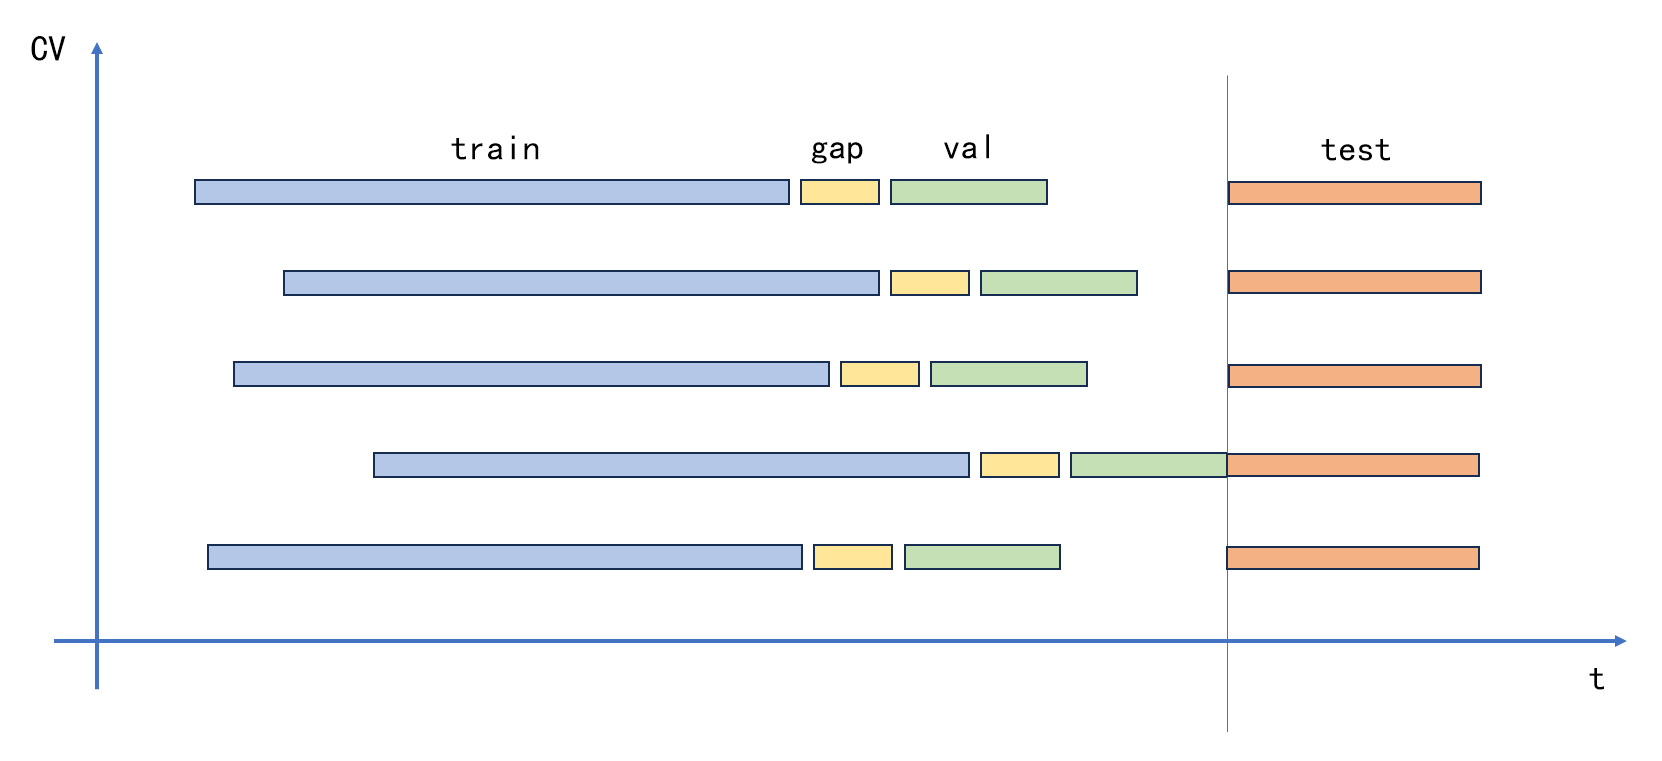
\includegraphics[width=0.8\textwidth]{Model/Demonstration of MC.jpg}
	\caption{Monte Carlo Cross Validation}
\end{figure}


The purpose of introducing a gap between the training and validation sets is to allow for a more realistic evaluation of the model's predictive capabilities and to mitigate overfitting. By simulating the scenario where predictions need to be made for future, unseen data, the model's ability to generalize can be properly assessed.



\subsection{Model optimization}
We mainly focus on selecting the best missing value handling technique and method for prediction generation. 

We employ different strategies to handle missing values based on whether only the target variable or the entire row is missing. For data with only missing target variables, we apply linear interpolation and direct deletion of the entire rows. For data with missing timestamps, we explore options of filling or not filling the time gap. Since LGBM treats NaN values as separate categories and in our application scenario, we believe that the missingness itself carries some information, we choose to fill the missing values with NaN. This preserves the missing timestamps as a distinct feature, and LightGBM can learn the impact of missing values on the target variable based on their presence or absence. For prediction generation, we select between using only the best iteration and taking average of all the iterations.

Hyperparameters of the model are shown in the table below. 


\begin{figure}[H]
	\centering
	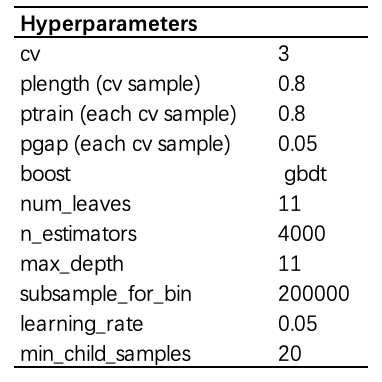
\includegraphics[width=0.4\textwidth]{Model/Hyperparameter.png}
	\caption{Hyperparameter list}
\end{figure}


\section{Performance evaluation}
To align with Kaggle's evaluation metirc, we evaluate our model by the weighted version of the Pearson correlation coefficient on the testing set and the result is shown below.

\begin{figure}[H]
	\centering
	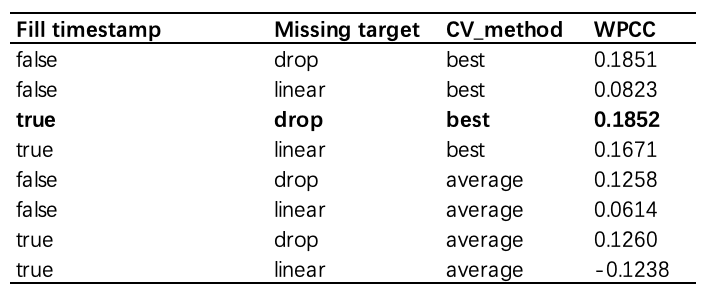
\includegraphics[width=0.8\textwidth]{Model/Result.png}
	\caption{Model performance}
\end{figure}

The best performing model employs timestamp imputation, excludes training data without the target variable, and generates predictions using only the best iteration. It achieves a weighted Pearson correlation coefficient of 0.1852. The weights and Pearson correlation coefficients for each cryptocurrency in each model are shown in the following table.

\begin{figure}[H]
	\centering
	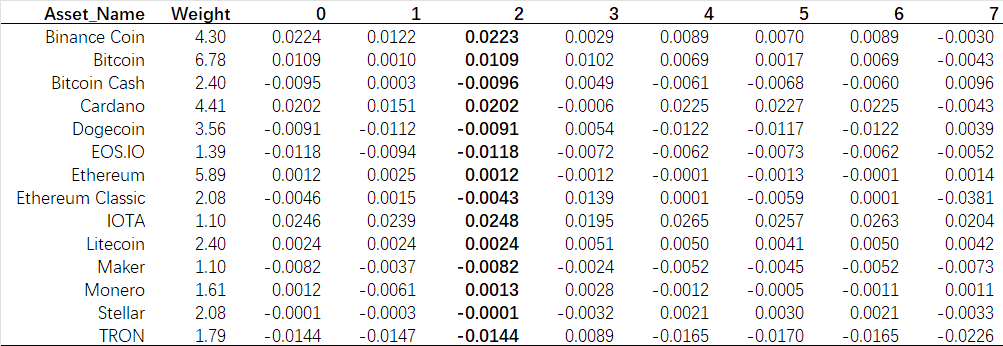
\includegraphics[width=1\textwidth]{Model/Detail for each asset.png}
	\caption{Pearson correlation coefficients for each cryptocurrency}
\end{figure}

\section*{References}

\medskip

\small


[1] Alessandro Ticchi, Andrew Scherer, Carla McIntyre, Carlos Stein N Brito, Derek Snow, Develra, dstern, James Colless, Kieran Garvey, Maggie, Maria Perez Ortiz, Ryan Lynch, Sohier Dane. (2021). G-Research Crypto Forecasting . Kaggle. https://kaggle.com/competitions/g-research-crypto-forecasting


[2] Picard, Richard R., and R. Dennis Cook. “Cross-validation of regression models.” Journal of the American Statistical Association 79.387 (1984): 575–583.

\section*{Group contribution}
Wang Jinyuan: Coding

Fu Yang: Presentation 

Luo Yuqing: Coding Support, Report writing and Latex formatting

Wang Tong: Coding Support

All members participate actively and equally contribute to this project.

\section*{Github link}
https://github.com/dboywjy/G_Research_Crypto_Forecasting/tree/dev_wjy/crypto

\end{document}

